

\begin{figure}[t]
    \centering
    \subfigure[PPO vs. GRPO]{%
        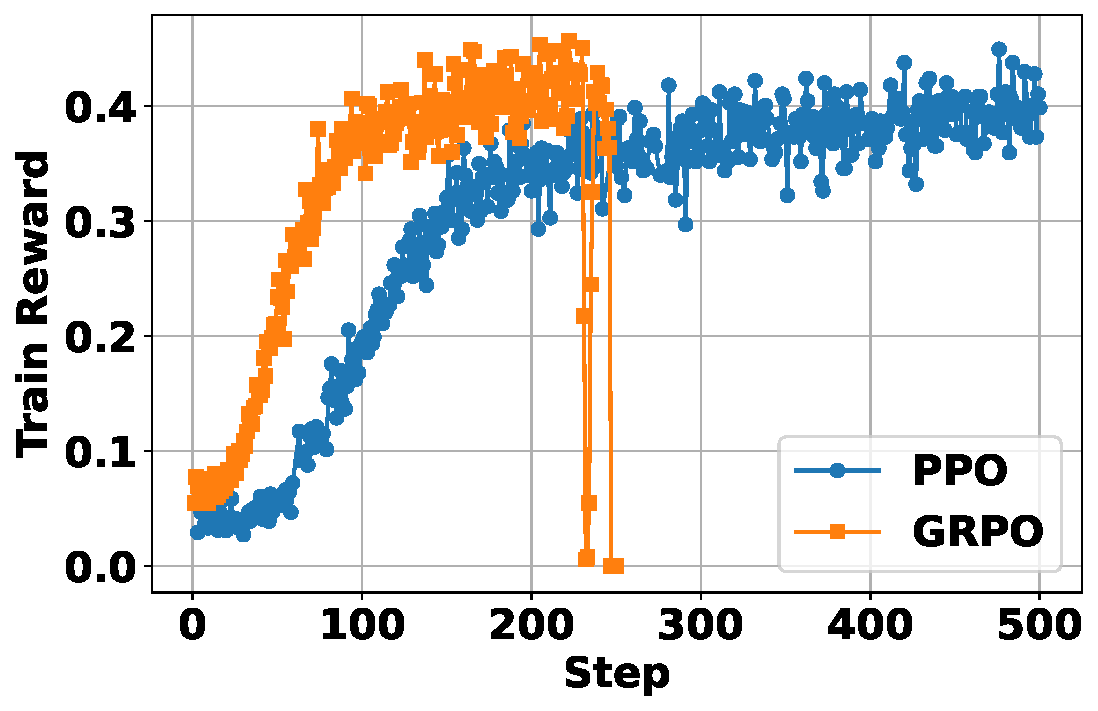
\includegraphics[width=0.225\textwidth]{figures/Search-R1_qwen-3b-base-ppo-grpo-new.pdf}
    }
    \subfigure[Base vs. Instruct]{%
        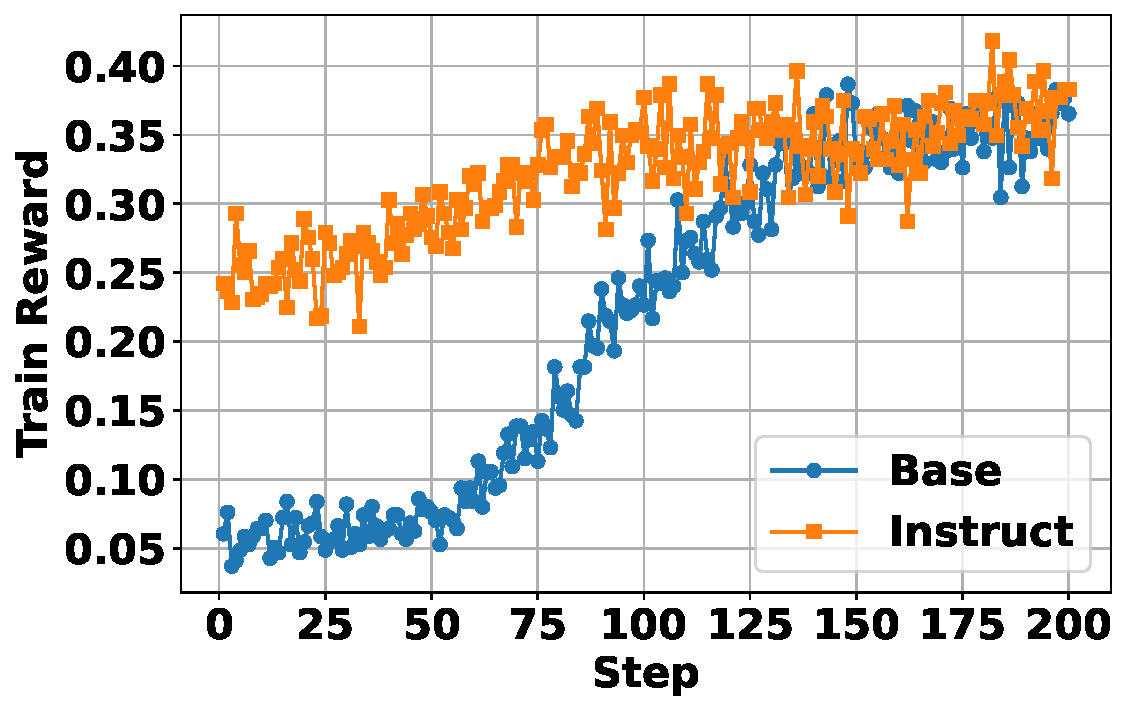
\includegraphics[width=0.225\textwidth]{figures/Search-R1_qwen-3b.pdf}
    }
    \subfigure[Response length]{%
        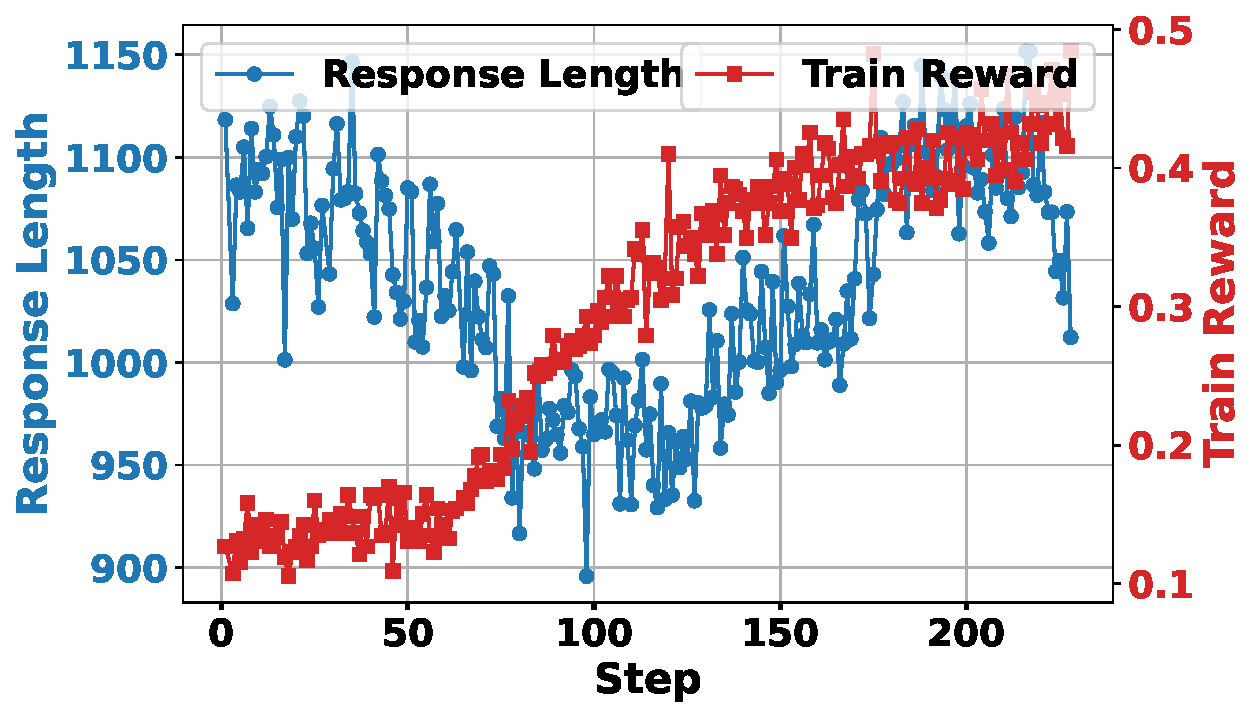
\includegraphics[width=0.255\textwidth]{figures/Search-R1_qwen-7b-response.pdf}
    }
    \subfigure[\# Valid search]{%
        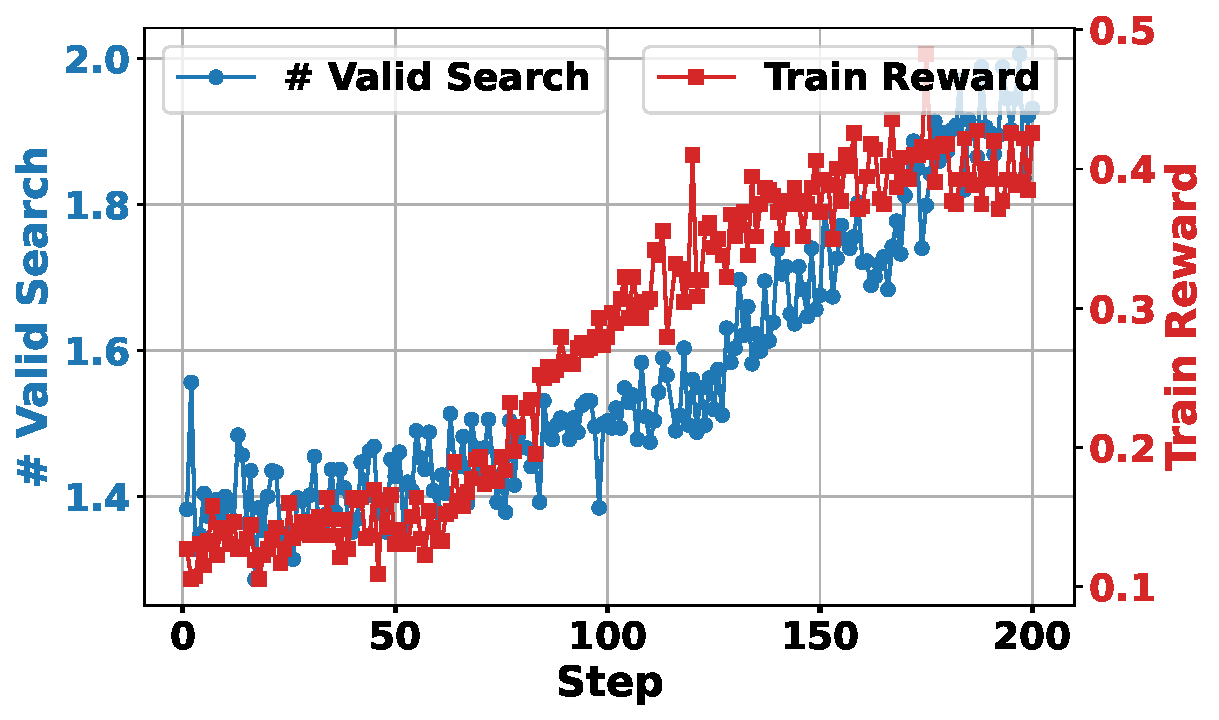
\includegraphics[width=0.25\textwidth]{figures/Search-R1_qwen-7b-valid-search.pdf}
    }
    % \subfigure[Loss mask]{%
    %     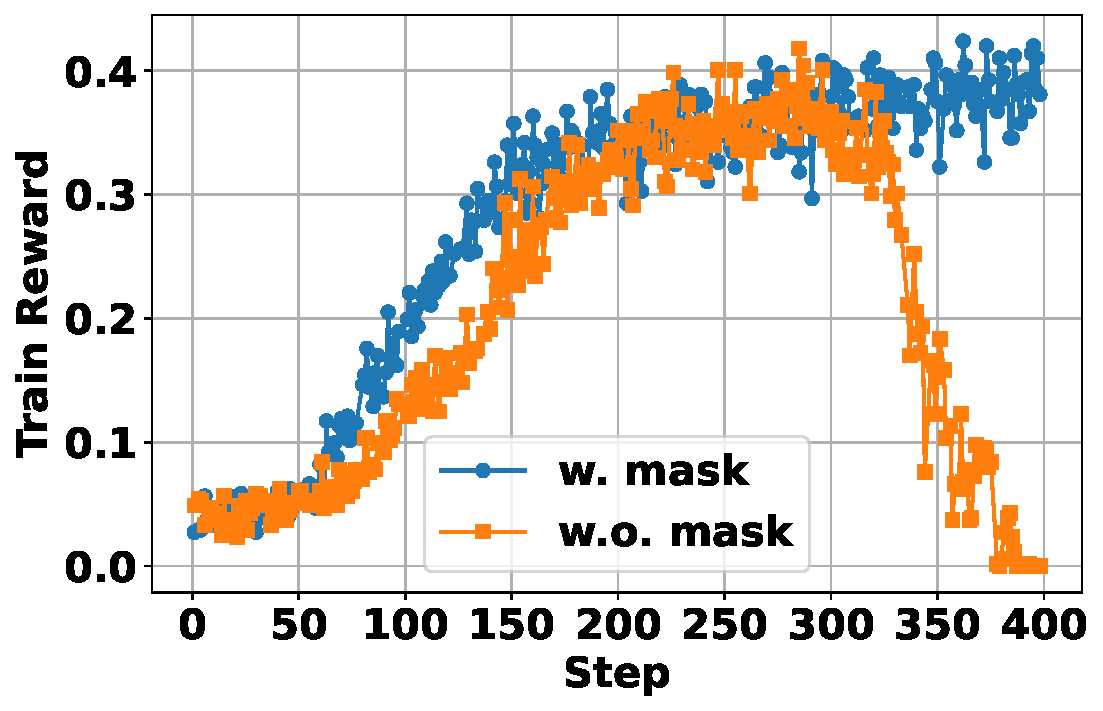
\includegraphics[width=0.225\textwidth]{figures/Search-R1_qwen3b-loss-mask.pdf}
    % }
    \vspace{-0.1in}
    \caption{
(a) PPO vs. GRPO: GRPO generally converges faster but may exhibit instability after trained
for a number of steps, whereas PPO provides more stable optimization but converges at a
slower rate.
(b) Base vs. Instruct LLM study: Instruction-tuned LLMs converge faster, but the final performance of both modles remains highly similar.
(c) Response length study: The response length exhibits a decrease-increase-stabilize trend throughout training, aligning with the overall performance trajectory of the LLM.
(d) \# Valid search study: As the training proceeds, the LLM learns to call search more.
% (d) Retrieved token loss masking study: Implementing retrieved token masking leads to greater LLM improvements, mitigating unintended optimization effects and ensuring more stable training dynamics.
}\label{fig:joint-study}
\vspace{-0.1in}
\end{figure}
